%%%%%%%%%%%%%%%%%%%%%%%%%%%%%%%%%%%%%%%%%%%%%%%%%%%%%%%%%%%%%%%%%%%%%%%%%%%%%%%
\documentclass[letterpaper, 10 pt, conference]{ieeeconf}  % Comment this line out
                                                          % if you need a4paper
%\documentclass[a4paper, 10pt, conference]{ieeeconf}      % Use this line for a4
                                                          % paper
\usepackage[utf8]{inputenc}  % Ng Edit for accents in spanish
\usepackage[spanish]{babel}  % Ng Edit for accents in spanish
\usepackage{hyperref}        % Ng Edit for adding urls
\usepackage{graphicx}        % Ng Edit for adding graphics
\usepackage{svg}
\IEEEoverridecommandlockouts                              % This command is only
                                                          % needed if you want to
                                                          % use the \thanks command
\overrideIEEEmargins
% See the \addtolength command later in the file to balance the column lengths
% on the last page of the document

\def\equationautorefname~#1\null{(#1)\null}%to use parenthesis in eqs.


% The following packages can be found on http:\\www.ctan.org
%\usepackage{graphics} % for pdf, bitmapped graphics files
%\usepackage{epsfig} % for postscript graphics files
%\usepackage{mathptmx} % assumes new font selection scheme installed
%\usepackage{times} % assumes new font selection scheme installed
%\usepackage{amsmath} % assumes amsmath package installed
%\usepackage{amssymb}  % assumes amsmath package installed

\title{\LARGE \bf
    Utilización de Múltiples Modelos de Redes Neuronales Convolucionales
    para la Detección de Rostros
}
\author{Pedro Luis González Roa, Pedro Oscar Pérez Murueta, Benjamín Valdés Aguirre,
José Antonio Cantoral Ceballos}

\begin{document}
    \maketitle
    \thispagestyle{empty}
    \pagestyle{empty}

    \begin{abstract}
        En los últimos años se ha demostrado la complejidad en la realización de
        algoritmos de detección y reconocimiento de rostros, ya que estos requieren de un alto
        nivel de abstracción porque existe un alto grado de similitud estructural entre los
        diferentes rostros. De esta manera, se requiere de la utilización de técnicas de
        \textit{deep learning}, cómo las \textit{redes neuronales convolucionales} (\textit{CNN}
        por sus siglas en inglés) para la extración de características o \textit{features} que 
        proporciona una imagen.  Estas técnicas requieren de un modelo sumamente complejo y una
        base de datos de gran tamaño para un entrenamiento exitoso que desempeñe correctamente en
        diferentes situación de iluminación, calidad de la imagen, perfil de la cara, entre otros.
        Cumplir con las características previamente mencionadas significa una gran inversión de
        recursos, la cual sólo empresas de tamaños inmensos son capaces de invertir.
        Por lo que se propone utilizar una combinación de diferentes \textit{CNN}'s previamente
        entrenadas con diferentes arquitecturas y bases de datos.
        Se espera que las diferentes perspectivas o características extraidas por cada modelo
        se complementen entre sí para tener una representación más completa (aunque
        más compleja) del rostro a analizar sin la necesidad de entrenar un modelo de complejidad
        tan grande como la previamente mencionada. Finalmente se utilizará esta representación
        más compleja para determinar los grupos de imágenes de acuerdo a las diferentes personas
        en la base de datos.
    \end{abstract}

    \section{Antecedentes}

    \subsection{Extracción de Características en Imágenes}
    % Image Clustering
    El reconocimiento facial se encuentra directamente relacionado con uno de los
    problemas que ha recibido mucha atención en las últimas tres décadas. El problema
    de agrupamiento de imágenes, también conocido como \textit{Image Clustering (IC)}
    por sus siglas en inglés, se centra en obtener una representación numérica sobre
    una imagen y agruparla con imágenes que tienen representaciones similares.
    \cite{CombiningCNN}

    % CNN
    Métodos de \textit{deep learning}, cómo las \textit{redes neuronales convolucionales},
    utilizan una casca de múltiples capas de unidades de procesamiento para extraer
    características específicas de las imágenes. Estas aprenden diferentes niveles de
    representación con cada capa de convolución que corresponden a los diferentes niveles
    de abstracción. Donde las primeras capas son capaces de reconocen y de detectar
    atributos de bajo nivel, similares a los modelos Gabor y SIFT (diseñados hace décadas);
    mientras que las capas más externas aprenden un nivel de abstracción más alto.
    Gracias a la variedad de niveles y filtros utilizados, los modelos de
    esta índole son capaces de tolerar a cierto nivel variaciones de ángulos,
    iluminación y calidad de la toma. \cite{Wang2021}

    \subsection{Reconocimiento de Rostros en la Actualidad}
    La detección de rostros consiste en tres fases principales:
    \begin{itemize}
        \item \textbf{Detección de rostro}: Aún cuando la detección de un rostro es trivial
            para los humanos, en términos de visión artificial no es una tarea sencilla. Esta
            tarea consiste en dado un vídeo o imágen, detectar y localizar un número
            desconocido de rostros (incluso si no hay alguno). Esta solución consiste en la
            segmentación, extracción y verificación de las posibles caras en un ambiente
            no controlado. \cite{FaceDetection2001}

        \item \textbf{Alineación del rostro}: Como segundo paso en este proceso, se alinea
            el rostro de acuerdo a coordenadas canónicas. \cite{Wang2021} Se han presentado
            varias propuestas, de las cuales las \textit{CNN} han obtenido buenos resultados.
            Para el proposito de este proyecto, se utilizará la propuesta de Zhang \cite{MTCNN}.
            La cual utiliza una \textit{CNN} para la detección y la alineación de los rostros
            en la misma secuencia.

        \item \textbf{Reconocimiento}: Este último paso consiste en procesar el rostro obtenido
            en los pasos anteriores. Primero se procesa el rostro con algoritmos para validar
            si consiste de un rostro verdadero y no modificado. Esta parte del proceso se conoce
            como \textit{anti-spoofing}. Después se utiliza técnicas de \textit{deep learning} cómo
            \textit{CNNs} para extraer las características que distinguen un individuo de otro.
            Finalmente se compara con cada uno de los registros de la base de datos de las
            personas identificadas para buscar un emparejamiento.
            Este proceso puede ser descrito de la siguiente manera: \cite{Wang2021}
                \[ M(F(P(I_1)), F(P(I_2))) \]
            En donde \textit{$I_1$} e \textit{$I_2$} son las imágenes por procesar, \textit{$P$}
            es la función de preprocesamiento, \textit{$F$} es la función para obtener las
            características del rostro, y \textit{$M$} es el cálculo de la distancia entre
            ambas representaciones y consecuentemente la confirmación si es un emparejamiento.
    \end{itemize}
    La extracción de estas representaciones no es un procedimiento trivial. Incluso utilizando
    las técnicas más avanzadas de \textit{deep learning}, es muy probable que el modelo se vea
    afectado por cambios en el contexto de la imagen. Estos cambios pueden ser la utilización
    de artefactos como lentes o cubrebocas; diferentes perfiles de la cara en donde se aprecia
    porciones importantes del rostro; ó incluso diferentes niveles de iluminación y calidad de la
    imágen. \cite{Bodini2019}

    \section{Trabajos Relacionados}

    \subsection{Combinación de Redes Neuronales Convolucionales Previamente Entrenadas}
    En previas investigaciones diferentes modelos de \textit{deep clustering algorithm}
    han demostrado un buen desempeño para pequeñas imágenes. Por otro lado, para
    obtener resultados exitosos en la agrupación de imágenes de mayor complejidad
    (cómo imágenes de objetos con estructuras complejas) es necesario la utilización
    de \textit{CNN}s previamente entrenadas para la extracción de características muy específicas.
    
    Existen una variedad de estos modelos, los cuales tienen un mismo objetivo pero aportan una
    perspectiva diferente gracias a variaciones dentro de las arquitecturas, funciones de
    activación y/ó base de datos utilizada para el entrenamiento. Para casos específicos un modelo
    puede tener mejor desempeño que otro en la obtención de características definitivas, pero en
    otro contexto puede tener un desempeño inferior. Guérin y coautores en la investigación
    \textit{'Combining pretrained CNN feature extractors to enhance clustering of complex natural images'}
    utilizan diferentes modelos \textit{CNN} para obtener resultados más constantes en la tarea de
    agrupación de imágenes complejas. Esto es gracias a que no se puede saber el modelo óptimo para
    cualquier situación (al menos de que se prueben todos), y al combinar diferentes modelos se
    obtiene una representación más completa y compleja. Esto es sacrificando una rápida respuesta
    a cambio de un resultado más fiable.\cite{CombiningCNN}


    \subsection{Modelo IE-CNN}
    An-Pint Song comprobó en su investigación \textit{'Similar Face Recognition Using the IE-CNN
    Model'} la importancia de tomar múltiples perspectivas sobre una misma imágen al realizar el
    reconocimiento de rostros. Este artículo menciona un fenómeno dentro de la investigación para
    el desarrollo de modelos de reconocimiento: siempre se utiliza la parte interna del rostro
    para el entrenamiento de los modelos. Lo cual no se apega completamente a cómo los humanos
    procesamos un nuevo rostro. Cuando es difícil determinar la comparación entre individuos,
    incrementamos nuestro enfoque en características específicas de la cara para disernir entre los
    dos diferentes rostros. \cite{Young1987} \cite{Andrews2010} Por lo que Song propone un modelo
    de \textit{CNN} que utiliza diferentes perspectivas enfocadas en partes estratégicas del rostro
    para obtener una representación mejorada. La cual obtuvo una mejora en los resultados de
    alrededor del 5\%. \cite{IECNN}

    \section{Planteamiento del Problema}
    % Diferentes situaciones afectan la fiabilidad de los modelos cnn
    Reiterando la problematica con la utilización de \textit{CNN} previamente mencionada
    la extracción de las características únicas de una cara para el reconocimiento facial
    es un reto no trivial por múltiples factores. Uno de estos es la posición del rostro,
    ya que es posible ocultar atributos clave que conllevan a una recolección incompleta
    de la información necesaria. Así mismo, el uso de artefactos como lentes o cubrebocas
    llevan a obstrucciones en dicha recolección. Por otro lado, las expresiones faciales
    pueden alterar la representación numérica, incluso cuando es la misma cara. Finalmente,
    los últimos factores que afectan son relacionados al ambiente, cómo la iluminación
    y la calidad de la cámara. \cite{Bodini2019}

    El diseño y entrenamiento de modelos lo suficientemente complejos que puedan desempeñarse
    correctamente en cualquier tipo de contexto requiere de una gran cantidad de recursos de
    \textit{hardware} y de una base de datos que incluya varias representaciones por cada uno
    de estos contextos. Incluso corporaciones gigantes han tenido problemas para resolver esta
    problematica en todos los casos posibles. Podemos tomar como ejemplo la situación en la que
    se encontró Apple, cuando su reconocimiento facial en sus dispositivos \textit{iphone} no
    era capaz de disernir correctamente entre individuos del país chino. \cite{Birchall2017}


    \section{Propuesta}
    % Modelo con mayor fiabilidad a coste de tiempo o utilización de hardware

    \subsection{Descripción de la propuesta}
    En esta investigación se propone utilizar múltiples modelos de redes neuronales convolucionales
    (\textit{CNN}) en combinación para obtener una representación de mayor complejidad pero de
    mayor precisión. Al igual que el modelo de Guérin \cite{CombiningCNN} se espera un aumento 
    en el tiempo de ejecución del programa, pero se busca resultados constantes durante contextos
    diferentes provenientes de bases de datos públicas.

    Así mismo, para acelerar el proceso de comparación entre imágenes se considera utilizar
    algoritmos de agrupamiento (\textit{clustering}) para realizar un mapa de las diferentes
    representaciones para cada rostro. De esta manera no es necesario comparar el rostro
    desconocido con cada una de las imágenes identificadas; sólo se predicirá el \textit{cluster} a
    cual pertenece.

    \subsection{Concatenación de Diferentes Representaciones (CC)}
    El acercamiento de concatenación consiste en, cómo su nombre lo dice, concatenar las
    diferentes representaciones obtenidas de cada modelo. En otras palabras, se agregan dimensiones
    por cada modelo que proporciona una perspectiva.
    
    Ya que se espera que entre más modelos utilizados la complejidad de tiempo crezca
    exponencialmente, se utilizará el algoritmo de reducción de dimensiones
    \textit{Principal Component Analysis (PCA)} para reducir el tiempo de procesamiento.

    \begin{figure}[ht]
        \centering
        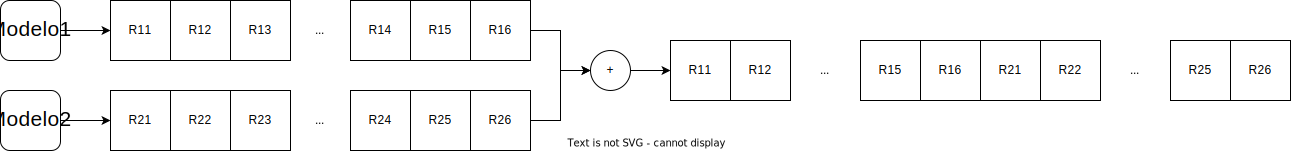
\includegraphics[width=8cm]{./figs/cc.png}
        \label{fig: Concatenación}
        \caption{Representación visual del acercamiento de concatenación.}
    \end{figure}

    \subsection{Utilización de Métodos de Consenso de Agrupamiento (MVEC)}
    Existen diferentes algoritmos e implementaciones para el agrupamiento de información. Aunque
    haya una gran variedad de estos algoritmos, muchos de estos encuentran soluciones apropiadas
    pero no óptimas. Estos convergen a un óptimo local y no a un óptimo global, aunque existe
    la pequeña posibilidad de que algunos sí llegan a este último (cómo por ejemplo: el algoritmo
    de \textit{k-means}. Ya que llegar a una solución óptima global es un poco aleatoria por la
    dependencia de la inicialización y distribución de las diferentes entradas, escoger un
    algoritmo de agrupación apto para la información persentada puede ser una tarea difícil. Para
    solucionar este problema, diferentes investigadores introdujeron el concepto de métodos de
    conjuntos para agrupamientos (\textit{Cluster Ensembles - CE} en inglés), ó también conocidos
    como métodos de consenso de agrupamiento (\textit{Consensus Clustering} en inglés). Los
    algoritmos de \textit{CE} combinan los diferentes resultados de agrupamiento para generar un
    agrupamiento final, sin necesitar acceso a los algoritmos o registros de información.
    \cite{Golalipour2021}

    \begin{figure}[ht]
        \centering
        \includegraphics[width=8cm]{./figs/mvec.png}
        \label{fig: MVEC}
        \caption{Representación visual del acercamiento de consenso.}
    \end{figure}

    Para el enfoque de este proyecto, utilizaremos la librería de Python proporcionada por Sano
    Takehiro \cite{Sano_ClusterEnsembles_2021}; con el algoritmo de \textit{Hybrid Bipartite Graph
    Formulation}. \cite{Fern2004}

    \subsection{Utilización de Agrupamiento de Múltiples Vistas (MVC)}
    En la era de \textit{Big Data}, se obtienen perspectivas diferentes de un mismo objeto desde
    una gran variedad de sensores. Estos sensores producen una salida de diferentes características
    entre sí, es decir son perspectivas que se complementan entre ellas para una representación
    más compleja del objeto observado. Por lo cual, ha surgido una tendencia a experimentar con
    algoritmos que puedan utilizar las diferentes dimensiones de cada vista para hacer predicciones
    más certeras.  En el ámbito de agrupamiento de información de múltiples vistas, ha incrementado
    en popularidad el algoritmo de Agrupación de vistas múltiples; \textit{Multi-View Clustering
    (MVC)} en inglés.

    Esta exhibición de propiedades heterógenas contiene un potencial de contener posibles
    conecciones entre ellas, las cuales pueden ser explotadas para desenmascarar características
    únicas de cada entrada de información. La idea principal de utilizar \textit{MVC} es
    particionar objetos de acuerdo a diferente criteria relacionada con estas conecciones de sus
    diferentes vistas. \cite{Yang2018}
    % Que es mvc
    % Por que mvc

    \subsection{Medición}
    % NMI
    Para evaluar el desempeño de este modelo de combinación se dividirá en dos etapas dicha
    evaluación:
    \begin{enumerate}
        \item Se dará la tarea de agrupar las imágenes de un número conocido y variable de
            personas. La composición de estos grupos será evaluada con la métrica
            \textit{Normalized Mutual Info (NMI)} \cite{NMI}.
        \item De un mapeo previamente realizado de un número conocido de personas, se agregarán
            más imágenes de personas incluidas en dicho agrupamiento y de otras no incluidas. Por
            cada imágen se evaluará si predijo correctamente la persona a la que pertenece o si
            es una persona nueva. Denotando el porcentaje de casos de falsos positivos,
            ya que es una métrica importante en los sistemas de seguridad biométricos.
        \item La diferencia de tiempo para realizar el agrupamiento entre cada uno de los
            acercamientos, así como también el tiempo que conlleva predecir una nueva imágen.
    \end{enumerate}

    \section{Resultados}
    % Fracaso mvc (Comparación de modelos de agrupamiento)
    % Resultados y consistencia de CC

    \section{Conclusiones}
    % Maybe worth it?

    \section{Futuras Aportaciones}
    % Utilizar más modelos como Inception
    % Deep Learning Clustering JULE
    % Entrenar modelos tapando partes estratégicas de la cara

    \bibliographystyle{ieeetr} % We choose the "plain" reference style
    \bibliography{refs} % Entries are in the refs.bib file
\end{document}
